% !TEX root = ../main.tex
\section{实验\chinese{section}}
\subsection{实验题目}
USCI-UART实验
\subsection{实验目的}
串口调试助手发送本人学号,单片机以查询方式接收并回传学号到串口调试助手,抓图并完成实验报告。
BRCLK = SMCLK = default DCO = 32 x ACLK = 1048576Hz;波特率= 9600;工作模式AM。
\subsection{实验仪器和设备}
计算机、开发板、示波器、信号源、电源、Code Composer Studio v5、串口调试助手等。
\subsection{实验步骤}
关闭看门狗,配置串口,设置波特率。从上位机通过串口将数据发送到单片机,再由单片机返回这些数据。
\subsection{程序清单}
\lstinputlisting{src/code/USCIUART2.c}
\subsection{实验结果记录与分析}
\begin{figure}[htbp]
	\centering
	\caption{USCIUART2}
	\label{USCIUART2}
	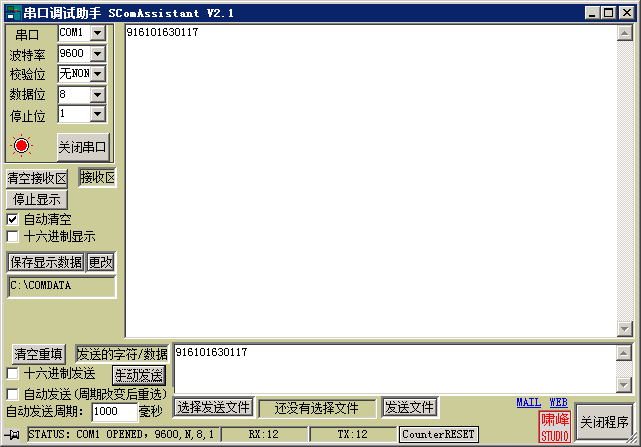
\includegraphics[width=10cm]{bitmap/png/USCIUART2.png}
\end{figure}
\subsection{遇到的问题与解决方法}
\begin{enumerate}
	\item RS232使用的DB9接口松动了,导致数据没有响应。
\end{enumerate}
